% !TEX root = thesis.tex

%%
%%
%% Discussion chapter
%%
%%

We are investigating the effectiveness of the DKD in estimating functions that return the incidence risk of chronic diseases. 
The DKD is computed by taking a kernel estimate of the disease incidence intensity and dividing by a kernel estimate of the population density at any given point.
We used several methods to estimate the error of the DKD estimate.
We ran several scenarios to examine how variations in the incidence risk function, the population, and the sample size affect the accuracy of the estimation. 


\begin{figure}[htbp]
  \centering
  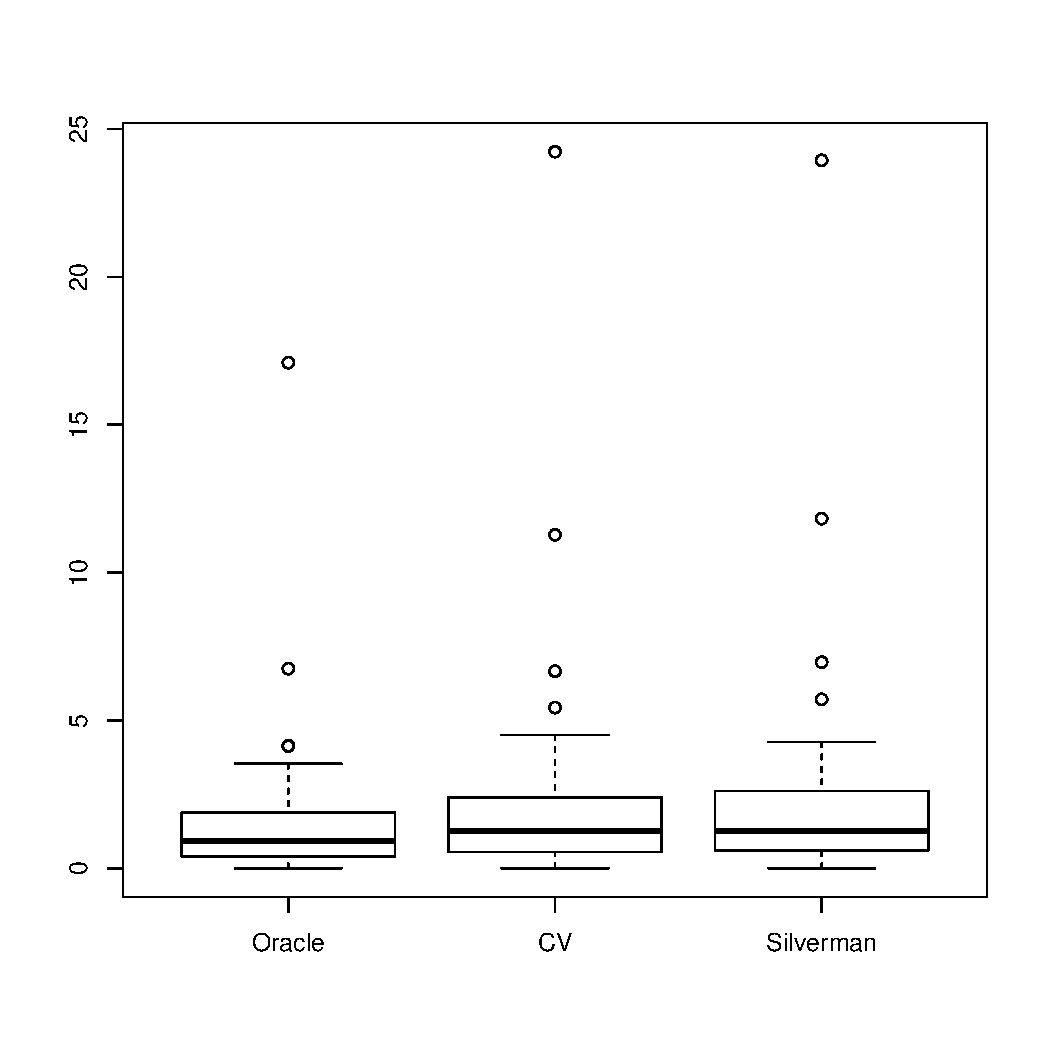
\includegraphics[width=0.45\textwidth]{results/by_overall/normalized-mise-boxplot}
  \caption{Overall distribution of \glsentryname{nmise}}
  \label{fig:discussion:overall_nmise_boxplot}
\end{figure}

\begin{figure}[htbp]
  \centering
  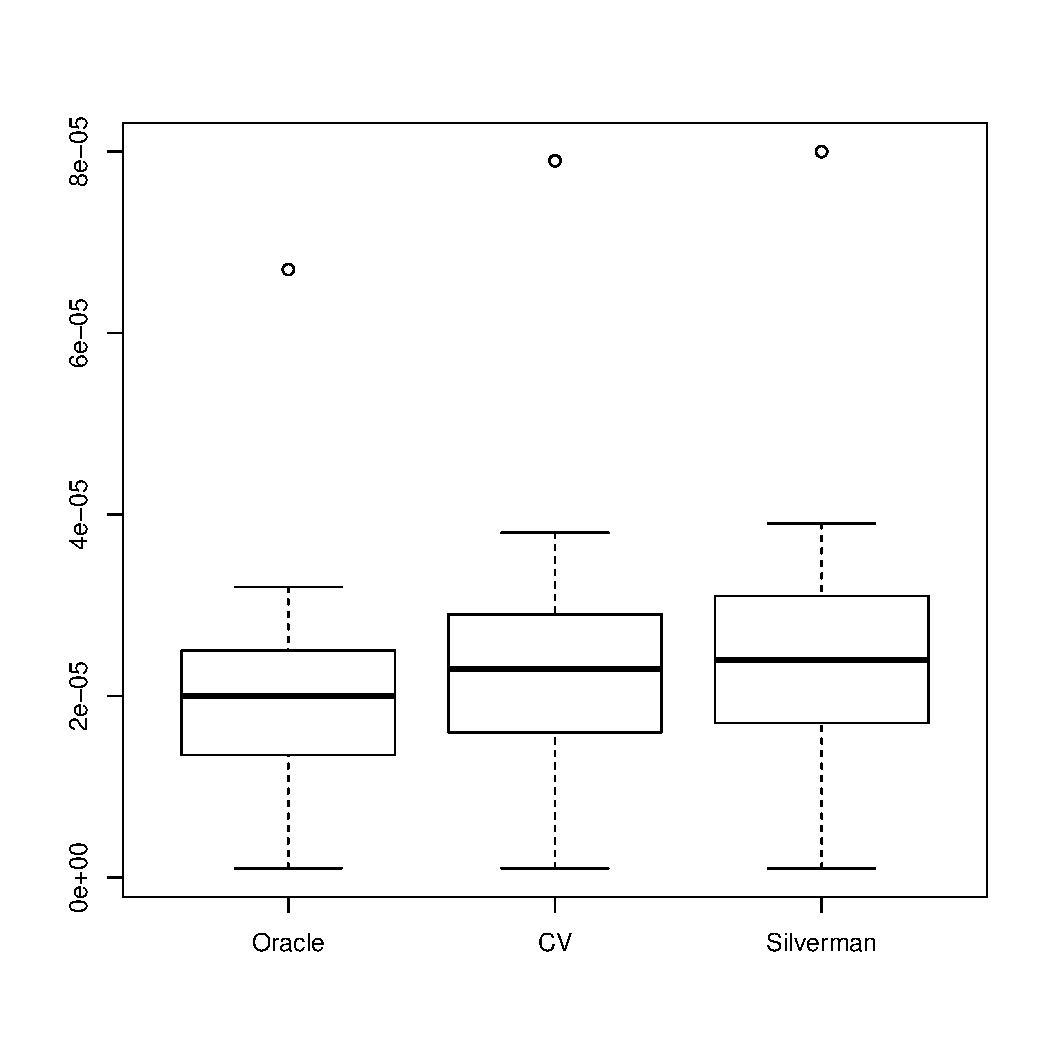
\includegraphics[width=0.45\textwidth]{results/by_overall/normalized-miae-boxplot}
  \caption{Overall distribution of \glsentryname{nmiae}}
  \label{fig:discussion:overall_nmiae_boxplot}
\end{figure}

\begin{figure}[htbp]
  \centering
  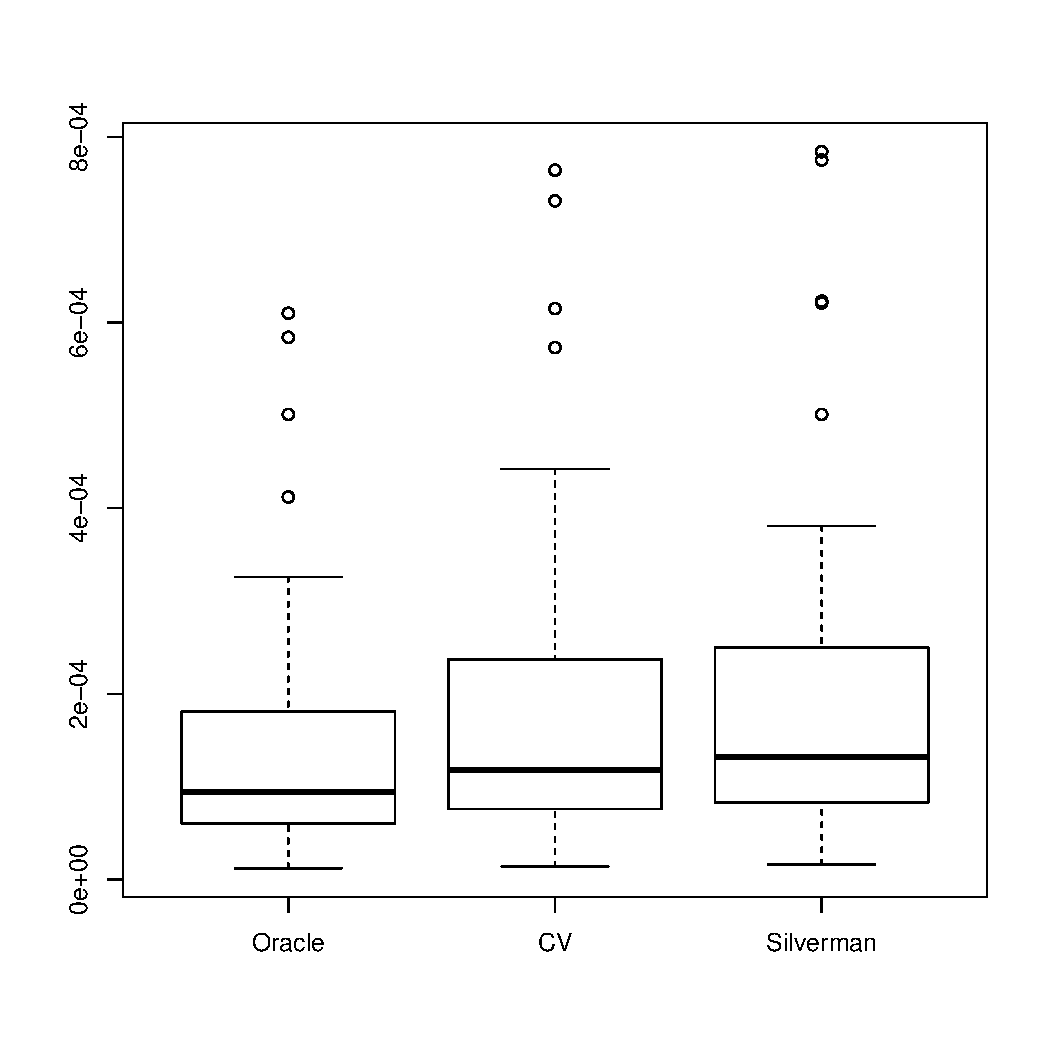
\includegraphics[width=0.45\textwidth]{results/by_overall/normalized-sup-error-boxplot}
  \caption{Overall distribution of \glsentryname{normalized supremum error}}
  \label{fig:discussion:overall_nsup_boxplot}
\end{figure}

\begin{figure}[htbp]
  \centering
  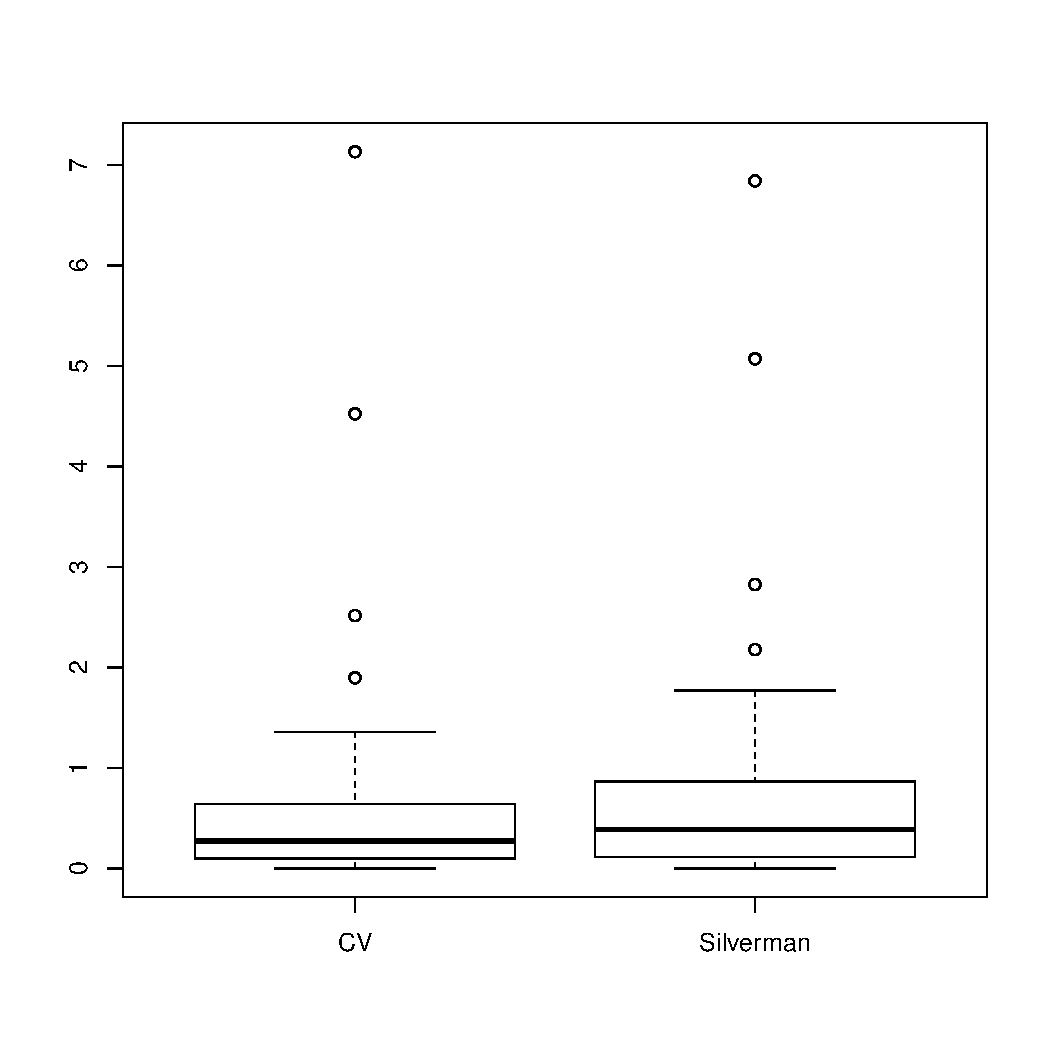
\includegraphics[width=0.45\textwidth]{results/by_overall/normalized-mise-diff-boxplot}
  \caption{Overall distribution of \glsentryname{nmise} difference from the \Glsentryname{oracle}}
  \label{fig:discussion:overall_nmise_diff_boxplot}
\end{figure}


\section{Gradient descent for cross-validation}
\label{sec:discussion:gradient_descent}

We attempted to speed up the cross-validation bandwidth selection by using gradient descent.
We found the gradient descent algorithm often resulted in severe oversmoothing,
as the cross-validation error would decrease slowly as the bandwidth increased.
This required a lot of manual tuning of the learning rate parameter, and so required re-running the experiment several times.
We added \textit{momentum} to our gradient descent implementation but it did not help in every case, and so we changed our strategy to the one described in \Cref{ch:method}.

\section{Accuracy using Silverman}

In \Cref{tab:mean_error_rates:p0.7_100_1.0_1h} we see that the accuracy measure \gls{mise} using the \gls{silverman} rule of thumb is even better than was obtained using the \gls{oracle}.
We tried to run with an additional experiment with 499 monte carlo simulations, and found that in this case the \gls{silverman} rule did not outperform the \gls{oracle}.

